\documentclass[12pt, a4paper]{article}

\usepackage{graphicx}
\setlength{\oddsidemargin}{0.5cm}
\setlength{\evensidemargin}{0.5cm}
\setlength{\topmargin}{-1.6cm}
\setlength{\leftmargin}{0.5cm}
\setlength{\rightmargin}{0.5cm}
\setlength{\textheight}{24.00cm} 
\setlength{\textwidth}{15.00cm}
\parindent 0pt
\parskip 5pt
\pagestyle{plain}
\graphicspath{ {./images/} }

\title{%
	Effect of mental imagery parameters on the risk of experiencing loneliness in a period of isolation \\
	\large Literature Review}
\author{}
\date{}

\newcommand{\namelistlabel}[1]{\mbox{#1}\hfil}
\newenvironment{namelist}[1]{%1
\begin{list}{}
    {
        \let\makelabel\namelistlabel
        \settowidth{\labelwidth}{#1}
        \setlength{\leftmargin}{1.1\labelwidth}
    }
  }{%1
\end{list}}

\begin{document}
\maketitle

\begin{namelist}{xxxxxxxxxxxx}
\item[{\bf Author:}]
	Mark Gabriel
\item[{\bf Supervisors:}]
	Dr. Julie Ji, Dr. Debora Correa, Dr. Wei Liu
\end{namelist}

\section{Abstract} The COVID-19 pandemic has forced a sudden change in society that we weren't fully prepared for.  Self-isolation and physical distancing has been imposed on everyone in varying degrees and the effect of it on people's mental wellbeing is an area of interest, especially if a second or third wave of the pandemic will require people to undergo isolation again. Certain members of the community are going to be affected more than others from this rapid disruption of the day-to-day because they are not getting the usual levels of social interaction they need or are used to to maintain a healthy mental wellbeing. It is in our interest to find which members of our community are at most risk with a method that is highly accessible given the physical restrictions that such a societal condition imposes. 

This study aims to be able to extract a risk level of loneliness from a person's free-text response to a scenario using natural language processing techniques. The mental imagery parameters of each response has been manually assessed and will be used to analyse what features of the corpus will be relevant in creating the model for determining a person's risk level. 

\section{Review of Literature}

\subsection{Mental Imagery}
Mental imagery is the simulation of perceptual experience \cite{Kosslyn2001} across sensory modalities. It has been strongly linked to depression \cite{Patel2005} which is our main area of interest. As detailed in Kosslyn et al's 2001 paper, the current techniques for measurements of a person's mental imagery involve visual tests, classification tasks, comparison tasks, questionnaires and interviews. 

The usage of machine learning and natural language processing has not yet been deeply explored in extracting mental imagery parameters, though theoretically, it would be most similar to the existing method of using interviews and analyzing a person's speech and selection of words to derive the wanted parameters, except with machine learning, the assessment would be automated rather than needing a trained professional to go through each case individually, which would be an expensive process that won't be easily scalable in an isolation scenario where potentially a huge percentage of people are affected.

Dr. Julie Ji's research on mental imagery, the experience of perception in the absence of external sensory input, shows that the person's quality of mental imagery-based simulations has a significant link to maintaining and amplifying emotional states \cite{conceptualandclinical}. In one study on mental imagery as a motivational amplifier to promote activities as a key treatment in depression \cite{motivationalamplifier}, the Motivational Imagery group reported higher levels of motivation, anticipated pleasure, and anticipated reward for the planned activities compared to the Activity Reminder control group and the No-Reminder control group.

\subsection{Named Entity Recognition}
We aim to be able to utilise the free-text responses of the survey to create a model that performs better than a regression model from the human-graded mental imagery parameters that predicts a person's risk of loneliness. To achieve this, the collected free-text responses have to be annotated with respect to the domain of interest. In our particular research area, it will be important to tag self actions (meditate, jog, sleep in, watch TV, etc) and interpersonal actions (call friend, video call with parents, have dinner at restaurant with partner) separately, which most pre-trained models aren't trained to do. Due to this, and also because we have a relatively small sample size, we have the luxury of using manual annotation to improve our data's richness and context.

In the paper Multilingual Twitter Sentiment Classification: The Role of Human Annotators by Mozetic et al, \cite{Mozeti__2016}, they find that the quality of classification models depends much more on the quality and size of training data than on the type of model trained. Human annotators can help us maximise our model's performance by ensuring good annotation quality, which can be done by setting an overlap value (the number of times a single corpus is annotated) of at least 2.


\begin{figure}
	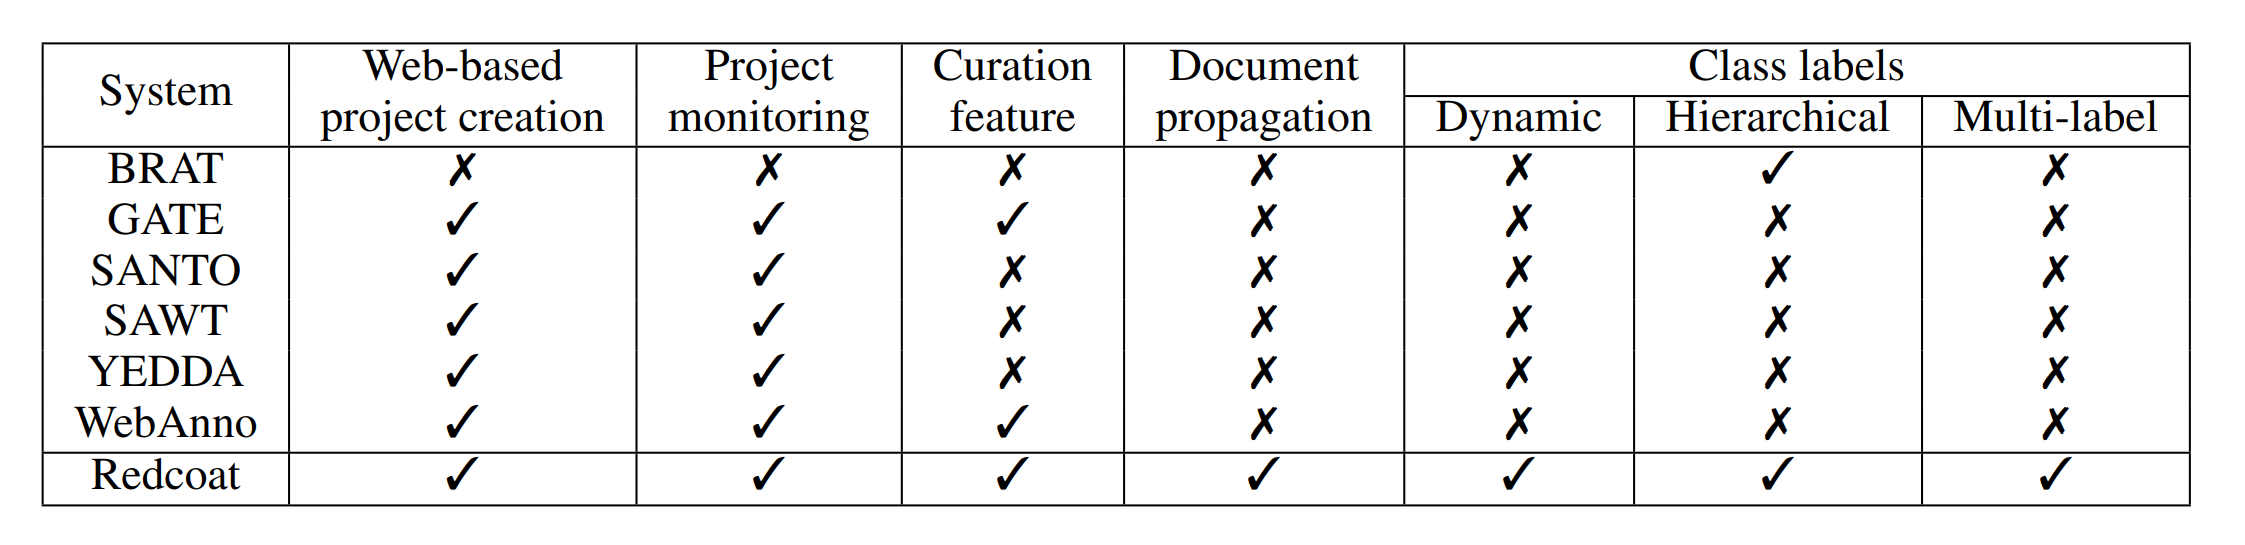
\includegraphics[scale=0.25]{annotating_tools}
	\caption{A comparison of existing annotation tools with Redcoat. Dynamic refers to the ability for any user to modify the class labels during annotation.}
	\label{annot_table}
\end{figure}

There are a lot of tools for data annotation available. Among these options are BRAT, GATE Teamware, WebAnno, SAWT, Yedda, SANTO and UWA's Redcoat. We can see a comparison of their features in Figure \ref{annot_table}. With research assistants to help out with our data as annotators, an important feature we are looking for in an annotating tool is the ability to propagate documents easily and for the tool to scale the workload automatically based on the number of annotators.  Redcoat \cite{stewart-etal-2019-redcoat} has been selected as the annotating tool for that reason, alongside being web-based and easy to set up and distribute. 

\subsection{Sentiment Analysis}
One of the mental imagery parameters we're concerned with is a person's emotional tone when they're describing what they think or see when they're given a scenario and a goal of starting lonely in an isolated setting and ending in a brighter, happier mental state. A person's emotional tone can be approximated with sentiment analysis techniques. XLNet has been used to identify optimism and pessimism in twitter messages by Alshahrani et al \cite{alshahrani2019xlnet}, which is similar to what we're trying to achieve. XLNet models are able to model negations and other semantic relationships by paying attention to key words, leading to a model accuracy of 96.45%. 

A point of discussion would be if our research problem would work better with basic sentiment analysis or aspect-based sentiment analysis. Normal sentiment analysis grades the emotional tone of the overall text, while aspect-based sentiment analysis goes through the text to identify various aspects and determines the corresponding emotional tone for each one. There isn't much available literature on when each of the techniques are relevant or when each of them should be used over the other, but the spirit of parsimony would lead us to towards using aspect-based sentiment analysis only if there are particular aspects in our research domain that we want to track individually. 

For the lack of literature on comparison between the two techniques on different domains, there is merit in trying both individually, or creating a model that uses both techniques in tandem and empirically comparing which technique works best for our research problem.

\subsection{Transfer Learning and XLNet}
Language is complex. In order to get reasonably performing models from scratch, one would need an extremely large dataset in addition to the computing power needed to process it. This is often impossible for many researchers, and a solution to this problem is transfer learning. Transfer learning is a machine learning technique where a model is trained on a particular problem, then reused in a similar domain to carry over the knowledge of the neural network. Depending on how different the pre-trained model is to your problem, Additional training needs to be done to finetune the model to your specific domain. \cite{ruder2019transfer}

Popular pre-trained NLP models include Google's BERT, Google and Carnegie Mellon University's XLNet, and Facebook's RoBERTa. All of these models are transformers which are deep learning models designed to handle sequential data using the concept of attention mechanisms. Attention mechanisms allow the model to access and use any previous states and utilises them based on relevance to the current node. \cite{vaswani2017attention} 

In particular, we want a pretrained model that is strong in sentiment analysis. Looking at Figure \ref{benchmarks} in the SST-2 column which stands for the Stanford Sentiment Treebank v2, we can see that XLNet \cite{yang2020xlnet} outperforms both BERT and RoBERTa in sentiment analysis on the SST-2 dataset.

While XLNet, BERT and RoBERTa all come from the same family of models, XLNet differs by introducing permutation language modelling, where all tokens are predicted in a random, permutated order rather than the traditional sequential order. This helps XLNet learn non-adjacent and bidirectional relationships between the words in the corpus. Secondly, XLNet uses Transformer-XLs as the base architecture which enables learning dependency beyond a fixed length without disrupting temporal coherence. \cite{dai2019transformerxl} Transformer-XLs, even without the permutation language modelling, has been shown to give performance increases in NLP tasks. 

\begin{figure}
	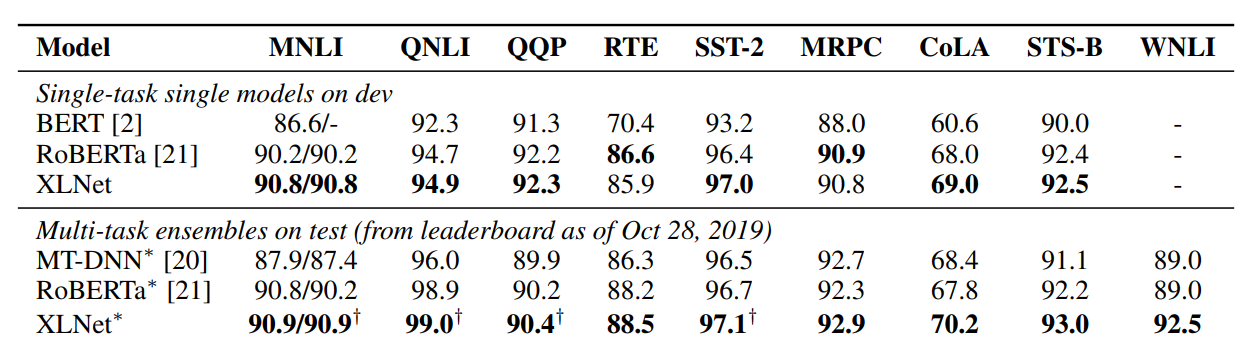
\includegraphics[scale=0.45]{benchmarks}
	\caption{Results on GLUE. * indicates using ensembles, and \dag  denotes single-task results in a multi-task row. All dev results are the median of 10 runs. The upper section shows direct comparison on dev data and the lower section shows comparison with state-of-the-art results on the public leaderboard.}
	\label{benchmarks}
\end{figure}

For the above reasons, and for the benchmarks set out in Figure \ref{benchmarks}, XLNet will be our pretrained model of choice. In addition, HuggingFace \cite{Wolf2019HuggingFacesTS} provides a transformer library that wraps all of these transformers for use with PyTorch or TensorFlow in a neat package that allows us to utilise the base XLNet model and the large XLNet model, alongside any other pretrained transformer model if we wish to make model comparisons. 

\bibliographystyle{plain}
\bibliography{literature_review}


\end{document}

